\documentclass[11pt]{article}

\usepackage[T1]{fontenc}
\usepackage[utf8]{inputenc}
\usepackage{lmodern}
\usepackage[margin=1in]{geometry}
\usepackage{amsmath,amssymb}
\usepackage{booktabs}
\usepackage{graphicx}
\usepackage{xcolor}
\usepackage[numbers,sort&compress]{natbib}
\usepackage[colorlinks=true,linkcolor=blue!50!black,citecolor=blue!50!black,urlcolor=blue!50!black]{hyperref}
\usepackage{microtype}

\newcommand{\todo}[1]{\textcolor{red}{[TODO: #1]}}
\newcommand{\pmsd}[2]{#1\,{\scriptsize$\pm$#2}}

\title{Asking Typed Questions about Radiographs with a Contrastive Decision Model:\\
Shared Heads, Paraphrase Robustness, and the Limits of Zero-Shot Transfer}

% Personal research; see research/ in the repository for the full record.
\author{Harvinder Singh\\
Independent researcher\\
\texttt{harvinderbhullar@gmail.com}}

\date{\today}

\begin{document}
\maketitle

\begin{abstract}
Contrastive language models (CLMs) answer typed questions about a state by scoring each candidate answer with the
cosine between a projected state embedding and a projected answer embedding, using frozen language-model encoders
and small trainable projection heads. We ask what such a model gains when its state is an image. We swap the state
tower for a frozen image encoder (Qwen3-VL-4B or MedSigLIP-448) with a newly trained head, keep the released text
action tower, and study fracture detection and seven further questions on the public FracAtlas radiograph dataset.
All choices are made on a validation split and the test split is evaluated once per experiment; one experiment is
pre-registered. Four findings hold on both encoders. (1)~For a binary question the CLM head matches a logistic
regression on the same frozen embedding (test AUROC 0.898 vs.\ 0.898 with MedSigLIP); with two fixed options the
text tower reduces to a fixed output direction, and random option vectors do as well. (2)~One head answers five
questions as well as one probe per question (macro AUROC 0.952 vs.\ 0.956). (3)~The text tower makes answers robust
to rewording: with unseen paraphrases of the options the head keeps macro AUROC 0.919 / 0.845, while random option
vectors fall to chance. (4)~A head trained from scratch cannot answer held-out questions zero-shot (0.496), although
MedSigLIP's own aligned text tower reaches 0.660 on the same questions. A pre-registered attempt to keep this
ability by aligning the head on text alone transfers some concepts to images without any image labels (fracture
0.741, above MedSigLIP's 0.659) but not the held-out view questions, and both pre-registered hypotheses are not
supported. We also report that a frozen logit scale makes the deployed head overconfident, corrected by validation
calibration (sensitivity 0.651$\to$0.835), and that 61 FracAtlas images have ambiguous labels or truncated files.
This is a research prototype, not a clinical tool.
\end{abstract}

\section{Introduction}

A contrastive language model (CLM) \citep{kwok2026clm} is trained so that the embedding of a \emph{state} (a
context, a question) lies close to the embedding of the \emph{action} taken in it. At inference a typed question
--- yes/no, multiple choice, or an ordered score --- becomes a closed set of candidate answers; each candidate is
embedded, scored by a scaled cosine against the state, and the softmax over candidates is the answer distribution.
Because states and actions are embedded independently by frozen encoders with small projection heads, embeddings
are cached and reused, which makes such a model fast to serve and cheap to fine-tune.

The released CLM is text-only. A natural extension is to let the state be an image: keep the text action tower,
so that questions and answers stay in natural language, and replace the state tower with a frozen image encoder and
a new head. This raises a simple question that the text setting does not answer: \emph{what does routing a
classification through text option embeddings buy, compared with a classifier on the same image features?} If the
text tower contributes nothing, a linear probe is the simpler model. If it contributes something --- robustness to
how a question is worded, or answers to questions never trained on --- the interface is worth its cost.

We study this on FracAtlas \citep{abedeen2023fracatlas}, a public set of 4{,}083 musculoskeletal radiographs with
fracture labels and metadata (body region, view, orthopedic hardware, several scans per image, fracture count). The
metadata lets us pose eight typed questions about every image and hold some out entirely. We use two encoders that
differ in kind: a general vision--language model (Qwen3-VL-4B \citep{qwen2025qwen3vl}, last-token pooling of a chat turn) and a medical
image encoder trained jointly with a text tower (MedSigLIP-448 \citep{sellergren2025medgemma}).

\paragraph{Contributions.}
\begin{itemize}
  \item A vision extension of CLM that swaps the state tower and keeps the released action tower, with serving
        support (image states routed to the head's own encoder, modality mismatches refused) and a validation
        calibration that corrects the overconfidence of a frozen logit scale (Sections~\ref{sec:method},
        \ref{sec:binary}).
  \item A controlled evaluation on two encoders: linear probes, per-question heads, random option vectors that
        remove the text tower's content, and MedSigLIP's own zero-shot text tower; validation-only selection and a
        single test evaluation per experiment (Section~\ref{sec:setup}).
  \item Four findings: the head equals a probe on a binary question; one head serves many questions at no cost;
        the text tower makes answers robust to paraphrase; zero-shot transfer to held-out questions fails for a
        head trained from scratch (Section~\ref{sec:results}).
  \item A pre-registered experiment that tries to preserve zero-shot ability by aligning the head on text alone;
        it transfers fractures, hardware and body regions to images without image labels, but not views
        (Section~\ref{sec:align}).
  \item Data-quality notes on FracAtlas: two images with ambiguous labels and 59 truncated JPEG files whose
        decoding creates a label shortcut (Section~\ref{sec:data}).
\end{itemize}

\section{Related work}

\paragraph{Contrastive image--text models.} CLIP \citep{radford2021clip} and SigLIP \citep{zhai2023siglip} align
images and text in one space and classify zero-shot by comparing an image with text prompts; LiT
\citep{zhai2022lit} trains the text tower against a locked image tower. Medical variants include ConVIRT
\citep{zhang2022convirt}, BiomedCLIP \citep{zhang2023biomedclip} and MedSigLIP \citep{sellergren2025medgemma}.
Our setting inverts LiT's: the \emph{text} side is locked (a text-trained CLM action tower) and only a projection
of a frozen image encoder is trained, typically from scratch.

\paragraph{Linear probes and zero-shot prompts.} Linear probes on frozen features are the standard measure of
representation quality \citep{kornblith2019better,radford2021clip}, and zero-shot prompt classifiers are known to
lag supervised probes on in-distribution labels. With a fixed set of options and a trainable projection, scoring
against text embeddings is a classifier whose output weights are fixed by the text encoder; our random-option
control makes this explicit.

\paragraph{Modality gap and text-only training.} Image and text embeddings of contrastive models occupy different
regions of the shared space \citep{liang2022mindthegap}, and models can be trained on text alone and applied to
images by exploiting the shared space \citep{nukrai2022capdec}. Our alignment experiment applies this idea to map
a medical image encoder into a text-trained CLM space.

\paragraph{Fracture detection.} FracAtlas \citep{abedeen2023fracatlas} provides classification, localisation and
segmentation labels; MURA \citep{rajpurkar2017mura} is a larger musculoskeletal abnormality dataset with study-level
labels. We do not aim at state-of-the-art fracture detection; fracture is the hard question in a set of typed
questions used to probe the CLM interface.

\paragraph{Calibration.} Neural classifiers are often overconfident \citep{guo2017calibration}; Platt scaling
\citep{platt1999probabilistic} fits a two-parameter logistic map on held-out data. We use it for the deployed head.

\section{Method}
\label{sec:method}

\begin{figure}[t]
  \centering
  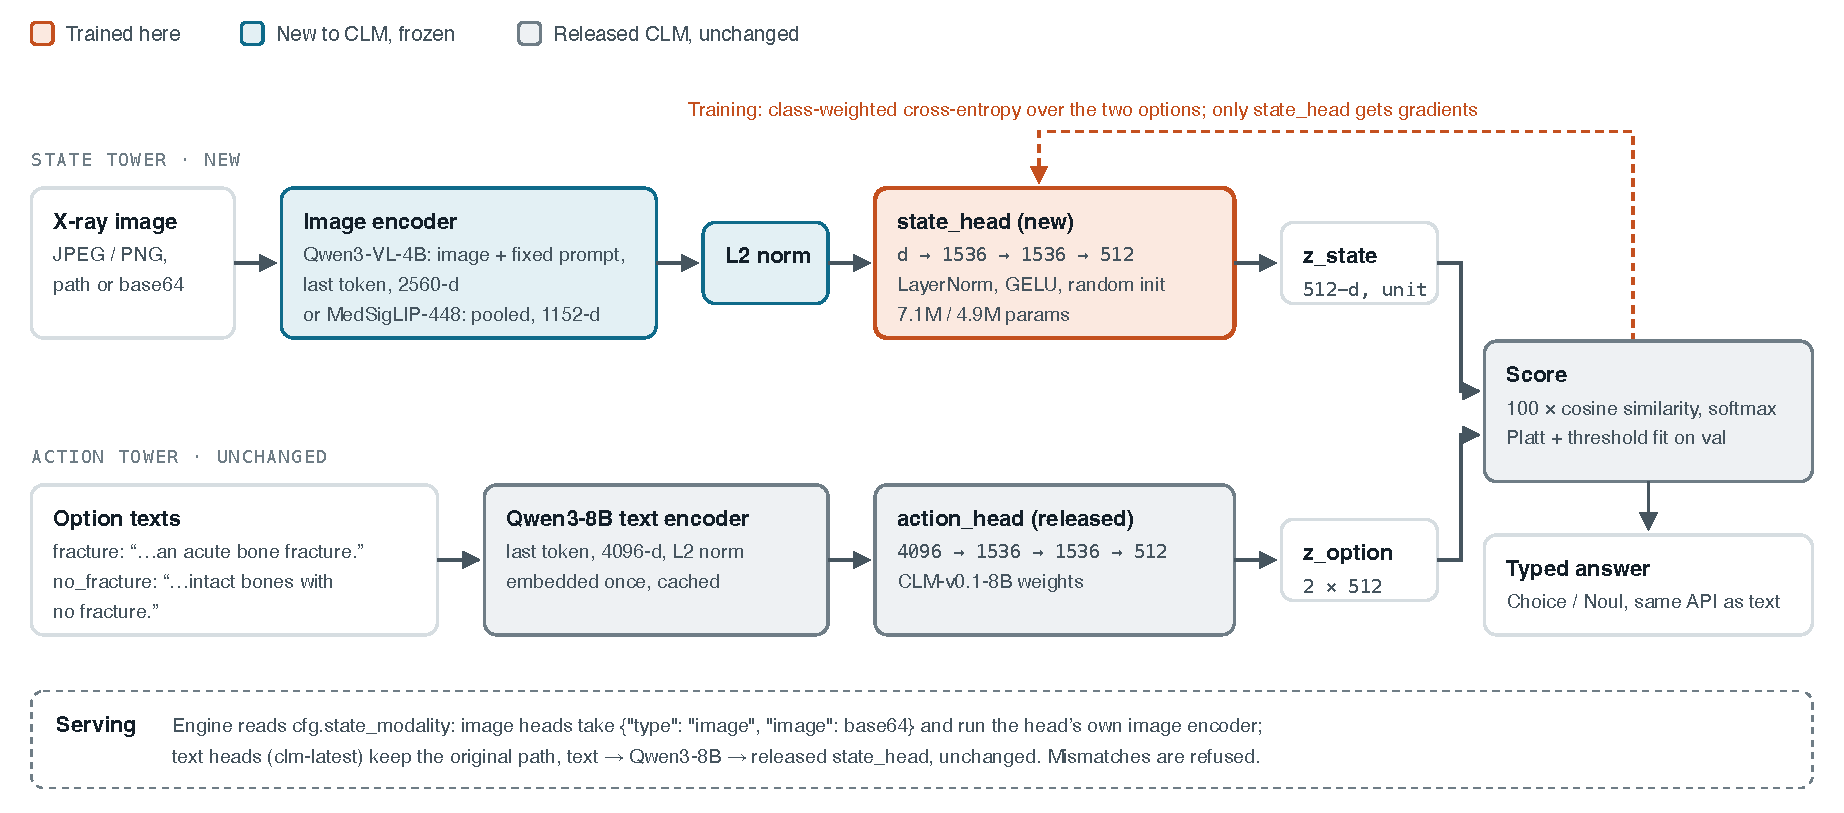
\includegraphics[width=\linewidth]{figures/clm_vision_arch.pdf}
  \caption{Vision extension of CLM. The state tower is new: a frozen image encoder and a trainable
  \texttt{state\_head}. The action tower is the released CLM one: option texts go through frozen Qwen3-8B and the
  released \texttt{action\_head}. A question's answer is the softmax of $100\times$ cosine over its options,
  optionally calibrated on validation data for serving.}
  \label{fig:arch}
\end{figure}

\paragraph{CLM scoring.} Let $e_s(\cdot)$ and $e_a(\cdot)$ be frozen encoders and $h_s$, $h_a$ projection heads
mapping to $\mathbb{R}^{512}$. For a state $s$ and a question $q$ with options $o_1,\dots,o_K$ (each embedded as its
text; yes/no options as \texttt{"true: \ldots"} / \texttt{"false: \ldots"}), the logits are
\begin{equation}
  \ell_k = \tau \,\cos\!\big(h_s(e_s(s)),\, h_a(e_a(o_k))\big), \qquad p(o_k \mid s) = \mathrm{softmax}_k(\ell),
\end{equation}
with $\tau=\min(\exp(\text{logit\_scale}),100)$; the released CLM-v0.1-8B head has $\tau=100$. The released heads
are three-layer MLPs ($4096\to1536\to1536\to512$, LayerNorm, GELU) over last-token embeddings of Qwen3-8B
\citep{qwen2025qwen3}.

\paragraph{Vision state tower.} We replace $e_s$ by a frozen image encoder and train a new $h_s$ of the same shape
from random initialisation: 7.1M parameters for Qwen3-VL-4B (2560-d input) and 4.9M for MedSigLIP (1152-d). For
Qwen3-VL-4B the state embedding is the final-norm hidden state of the last token of a chat turn containing the image
(longest side capped at $1024^2$ pixels) and the fixed text ``Radiograph for fracture assessment.''; for MedSigLIP
it is the pooled image embedding. Embeddings are L2-normalised and cached. $e_a$, $h_a$ and $\tau$ stay frozen, so
option embeddings are computed once. Inputs are standardised with training statistics; the affine map is folded
into the head's first linear layer, so checkpoints keep the CLM format.

\paragraph{Training objective.} We minimise class-weighted cross-entropy over each question's own options. In-batch
InfoNCE, used to train CLM, is unsuitable here: with two classes, images with the same label would be pushed apart
as negatives. For several questions the loss is averaged over the training questions, and one image embedding
answers every question (the question text does not reach the image encoder).

\paragraph{Calibration for serving.} With $\tau=100$ frozen, raw probabilities are extreme. For deployment we fit,
on validation data, Platt scaling of the logit difference, $p=\sigma(a(\ell_{+}-\ell_{-})+b)$, and a decision
threshold maximising Youden's $J$ \citep{youden1950index}, store both in the checkpoint, and apply them when a
question's options match the fitted pair. AUROC is unchanged; the decision and the probabilities change.

\paragraph{Text-only alignment.} To keep zero-shot ability (Section~\ref{sec:align}) we exploit MedSigLIP's
shared image--text space. On a corpus of radiograph descriptions $t$, we train $h_s$ so that
$h_s(\mathrm{SigLIP}_{\text{text}}(t))$ matches the frozen CLM action embedding $h_a(e_a(t))$ of the same sentence,
with symmetric InfoNCE \citep{oord2018cpc} at scale 100 over batches of 256 sentences. Applied to an image
embedding, the head should land near the action embeddings of descriptions that match the image. Optionally the
alignment loss is kept, with weight $\lambda$, while fine-tuning on labelled questions.

\section{Experimental setup}
\label{sec:setup}

\subsection{Data}
\label{sec:data}

FracAtlas \citep{abedeen2023fracatlas} (CC BY 4.0) contains 4{,}083 radiographs of hand, leg, hip and shoulder,
717 of them fractured in the cleaned set. Two data problems were found (Table~\ref{tab:cleaning}). Two images appear
in both class folders; the annotation file marks them fractured but their bounding-box files are empty. Fifty-nine
JPEG files are truncated in the official archive (checksum verified); all are non-fractured and consecutive
(IMG0004028--IMG0004347). Decoding them anyway fills up to 54 bottom rows with flat grey, a label shortcut, so they
are removed. Without patient identifiers the split is per image: 70/15/15, stratified by label and body region,
seed 20261004, giving 2{,}813 / 609 / 600 images with 499 / 109 / 109 fractured. Consecutive images often show
several views of one study, so a patient can appear in more than one split; test numbers are optimistic for unseen
patients. Image size correlates with the label (29.1\% fractured above one megapixel vs.\ 16.5\% below), but a
classifier on log pixel count reaches only 0.528 test AUROC.

\begin{table}[t]
  \centering\small
  \caption{Data cleaning of FracAtlas.}
  \label{tab:cleaning}
  \begin{tabular}{p{7.2cm}rp{5.2cm}}
    \toprule
    Issue & Images & Action \\
    \midrule
    In both class folders, empty fracture annotation & 2 & dropped (ambiguous label) \\
    Truncated JPEG in the official archive (all non-fractured) & 59 & dropped after splitting (grey-band shortcut) \\
    \midrule
    Used & 4{,}022 & 717 fractured (17.8\%) \\
    \bottomrule
  \end{tabular}
\end{table}

\subsection{Questions}

Eight typed questions are derived from the labels (Appendix~\ref{app:questions}): fracture (choice, 2 options),
body region (choice, 5), frontal / lateral / oblique view (three yes/no), orthopedic hardware (yes/no), several scans
in one image (yes/no), and fracture count (score: 0, 1, 2+). Every option has three wordings: wording~0 is used for
training, wordings~1 and~2 only to test robustness to paraphrase. In the multi-question experiments the three view
questions are \emph{held out}: never trained on and never used for model selection. Hardware overlaps with fracture
(97 of 99 hardware images are fractured), and region, view and several-scans are easy for every method.

\subsection{Methods compared}

\begin{itemize}
  \item \textbf{CLM head}: the vision state head of Section~\ref{sec:method}.
  \item \textbf{Linear probe}: standardised logistic regression with balanced class weights (multinomial for more
        than two options), $C$ chosen on validation from $10^{-5}$ to $10^{1}$.
  \item \textbf{Random option vectors}: the CLM head trained with each option text replaced by a fixed random unit
        vector; it isolates the content of the text tower.
  \item \textbf{One CLM head per question}: the multi-question control for sharing.
  \item \textbf{MedSigLIP text tower}: zero-shot scoring of the cached image embedding against MedSigLIP's own text
        embedding of each option description, with no training.
  \item \textbf{Resolution only}: logistic regression on log pixel count (shortcut check).
\end{itemize}

\subsection{Protocol and metrics}

Every hyperparameter, logistic-regression $C$, decision threshold and calibration map is chosen on the validation
split. Each experiment's test split is evaluated once, after selection; evaluation scripts were first run with
validation data standing in for test. CLM heads are trained with three seeds and reported as mean $\pm$ standard
deviation. We report AUROC (macro one-vs-rest for questions with more than two options) with 95\% stratified
bootstrap intervals \citep{efron1993bootstrap} (2{,}000 resamples), sensitivity and specificity at the validation
Youden threshold, sensitivity at 90\% specificity, expected calibration error (ECE, 15 bins) raw and after
validation Platt scaling, and balanced accuracy. CLM-versus-probe differences use a paired bootstrap over the same
resamples. The alignment experiment was pre-registered before any run (Section~\ref{sec:align}).

\subsection{Implementation and compute}

All experiments ran on one Apple M5 Pro laptop with 24\,GB unified memory, using PyTorch 2.10 on the Apple GPU
(MPS) and \texttt{transformers} 5.17; Qwen3-VL-8B did not fit, so the released 4096-d state head could not warm-start
a vision head. Embedding all 4{,}022 images took 39\,min with Qwen3-VL-4B (fp16; 3.8 images/s at $373\times454$,
0.26 images/s for the 351 large scans) and 9\,min with MedSigLIP; option texts were embedded by Qwen3-8B in bf16.
A CLM head trains in seconds (median 5\,s); each sweep took about 12--15\,min. Hyperparameter grids are in
Appendix~\ref{app:hparams}; code, logs and a claims ledger linking every number to its source file and commit are
in the repository.

\section{Results}
\label{sec:results}

\subsection{A binary question: the CLM head equals a linear probe}
\label{sec:binary}

\begin{table}[t]
  \centering\small
  \caption{Fracture detection on the test split (600 images, 109 fractured). CLM rows: mean $\pm$ sd over three
  seeds. Thresholds and Platt scaling fit on validation.}
  \label{tab:binary}
  \setlength{\tabcolsep}{4pt}
  \begin{tabular}{lcccccc}
    \toprule
    Method & AUROC [95\% CI] & Sens. & Spec. & Sens.@90\%Spec. & ECE & ECE (Platt) \\
    \midrule
    Resolution only & 0.528 [0.491, 0.566] & 0.147 & 0.916 & 0.147 & 0.317 & 0.003 \\
    Linear probe, Qwen3-VL-4B & 0.890 [0.850, 0.927] & 0.817 & 0.849 & 0.725 & 0.159 & 0.036 \\
    CLM head, Qwen3-VL-4B & \pmsd{0.887}{0.012} & 0.820 & 0.778 & 0.697 & 0.129 & 0.043 \\
    Linear probe, MedSigLIP & 0.898 [0.860, 0.931] & 0.771 & 0.859 & 0.743 & 0.118 & 0.020 \\
    CLM head, MedSigLIP & \pmsd{0.898}{0.012} & 0.810 & 0.838 & 0.761 & 0.088 & 0.029 \\
    \bottomrule
  \end{tabular}
\end{table}

\begin{figure}[t]
  \centering
  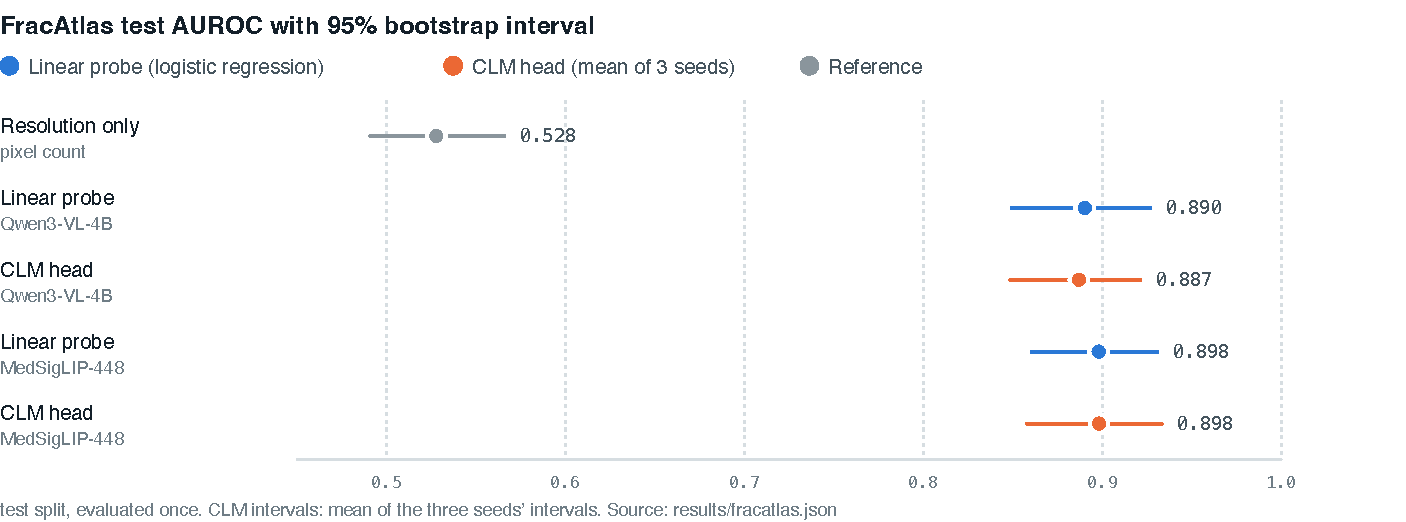
\includegraphics[width=0.85\linewidth]{figures/fracatlas_auroc.pdf}
  \caption{Test AUROC for fracture detection with 95\% bootstrap intervals.}
  \label{fig:auroc}
\end{figure}

Table~\ref{tab:binary} and Figure~\ref{fig:auroc} show that the CLM head matches the linear probe: the paired
difference is $-0.003$ [$-0.026$, $+0.021$] with Qwen3-VL-4B and $+0.000$ [$-0.020$, $+0.020$] with MedSigLIP.
MedSigLIP's head looked better on validation (0.918 vs.\ 0.898), an edge that did not survive the single test
evaluation; it was selection noise from choosing among 48 runs on one validation split. Replacing the Qwen3-8B
option embeddings by random vectors gives the same AUROC (Table~\ref{tab:ablation}): with two options the logit
difference is $\tau\,\hat z^{\top}(a_{+}-a_{-})$, so the text tower contributes one fixed direction and the head
acts as an MLP classifier. Other ablations (trainable scale, no input standardisation, no class weights) change
AUROC by at most 0.009.

\begin{table}[t]
  \centering\small
  \caption{Ablations of the CLM head, test AUROC (mean $\pm$ sd over three seeds).}
  \label{tab:ablation}
  \begin{tabular}{lcc}
    \toprule
    Variant & Qwen3-VL-4B & MedSigLIP \\
    \midrule
    CLM head (lr $3\times10^{-5}$, weight decay 0.1) & \pmsd{0.887}{0.012} & \pmsd{0.898}{0.012} \\
    Trainable logit scale & \pmsd{0.881}{0.003} & \pmsd{0.903}{0.008} \\
    No input standardisation & \pmsd{0.890}{0.001} & \pmsd{0.889}{0.007} \\
    No class weights & \pmsd{0.881}{0.012} & \pmsd{0.896}{0.003} \\
    Random option vectors & \pmsd{0.871}{0.011} & \pmsd{0.894}{0.007} \\
    \bottomrule
  \end{tabular}
\end{table}

\paragraph{Serving: a frozen scale makes the head overconfident.} With $\tau=100$ about 90\% of validation
probabilities lie below 0.01 or above 0.99, and the best cut is near $p\approx10^{-5}$. The plain answer
(the more probable option) therefore misses many fractures. Validation calibration fixes this for the deployed
seed-0 heads (Table~\ref{tab:served}). Accuracy falls because it rewards answering ``no fracture'' when 82\% of
images are intact (always answering ``no fracture'' scores 0.818); a trainable scale does not fix the problem, since
it only drifts to about 95--99.

\begin{table}[t]
  \centering\small
  \caption{Deployed heads (seed 0) on test: plain answer ($p>0.5$) vs.\ validation-calibrated decision.}
  \label{tab:served}
  \begin{tabular}{lccccccc}
    \toprule
    & & \multicolumn{3}{c}{Plain answer} & \multicolumn{3}{c}{Calibrated} \\
    \cmidrule(lr){3-5}\cmidrule(lr){6-8}
    Head & AUROC & Sens. / Spec. & Acc. & ECE & Threshold & Sens. / Spec. & ECE \\
    \midrule
    MedSigLIP & 0.889 & 0.651 / 0.963 & 0.907 & 0.085 & 0.112 & 0.835 / 0.772 & 0.040 \\
    Qwen3-VL-4B & 0.900 & 0.596 / 0.937 & 0.875 & 0.116 & 0.173 & 0.798 / 0.809 & 0.032 \\
    \bottomrule
  \end{tabular}
\end{table}

\subsection{Many questions: sharing, paraphrase and zero-shot}
\label{sec:multiq}

\begin{table}[t]
  \centering\small
  \caption{Multi-question experiment, test macro AUROC. Five trained questions; three held-out view questions
  answered zero-shot. CLM rows: mean $\pm$ sd over seeds (the text quotes the seed-averaged head, 0.496 for
  MedSigLIP held out). Rows marked $^{\dagger}$ were trained on the view labels (supervised reference).}
  \label{tab:multiq}
  \begin{tabular}{lcccc}
    \toprule
    & \multicolumn{2}{c}{MedSigLIP} & \multicolumn{2}{c}{Qwen3-VL-4B} \\
    \cmidrule(lr){2-3}\cmidrule(lr){4-5}
    Method & Trained & Held out & Trained & Held out \\
    \midrule
    One CLM head, all questions & \pmsd{0.952}{0.004} & \pmsd{0.488}{0.014} & \pmsd{0.951}{0.004} & \pmsd{0.495}{0.012} \\
    Random option vectors & \pmsd{0.953}{0.003} & \pmsd{0.465}{0.114} & \pmsd{0.946}{0.003} & \pmsd{0.495}{0.062} \\
    One CLM head per question & \pmsd{0.957}{0.002} & 0.978$^{\dagger}$ & \pmsd{0.950}{0.004} & 0.954$^{\dagger}$ \\
    One linear probe per question & 0.956 & 0.974$^{\dagger}$ & 0.948 & 0.951$^{\dagger}$ \\
    MedSigLIP text tower, no training & 0.811 & 0.660 & -- & -- \\
    \midrule
    CLM head, paraphrase 1 / 2 & 0.919 / 0.845 & & 0.915 / 0.844 & \\
    Random vectors, paraphrase 1 / 2 & 0.449 / 0.460 & & 0.501 / 0.545 & \\
    MedSigLIP text tower, paraphrase 1 / 2 & 0.778 / 0.736 & & -- & \\
    \bottomrule
  \end{tabular}
\end{table}

\begin{figure}[t]
  \centering
  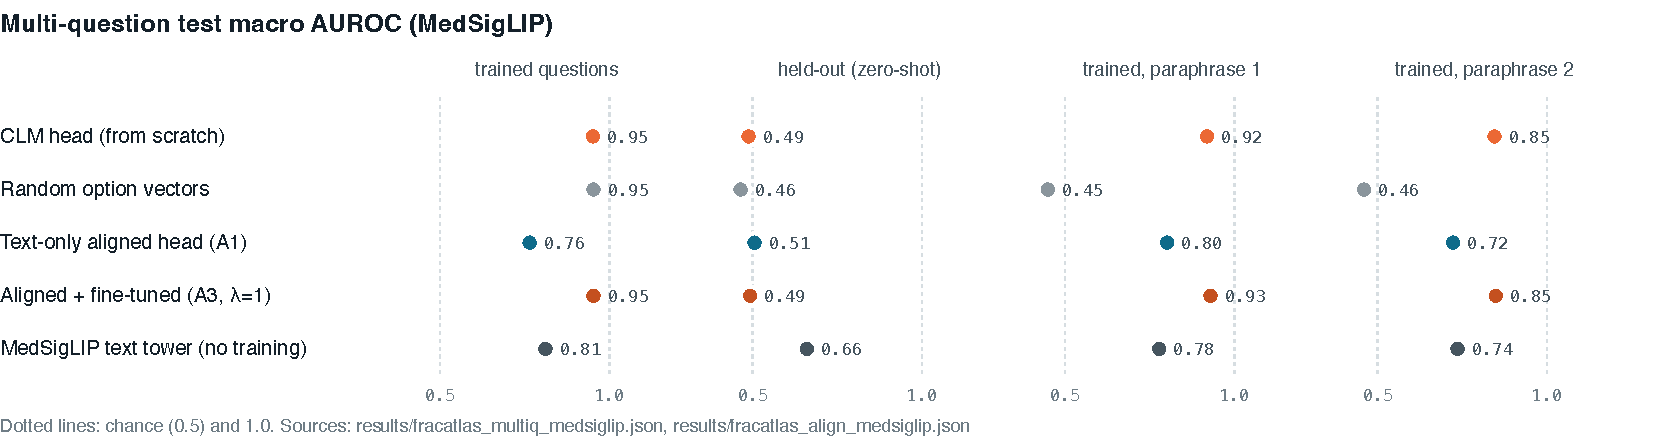
\includegraphics[width=\linewidth]{figures/fracatlas_zero_shot.pdf}
  \caption{Multi-question test macro AUROC with MedSigLIP, including the alignment experiment
  (Section~\ref{sec:align}). Paraphrase columns use option wordings never seen in training.}
  \label{fig:zeroshot}
\end{figure}

Table~\ref{tab:multiq} and Figure~\ref{fig:zeroshot} summarise three results.

\paragraph{Sharing one head costs nothing.} One head answers the five trained questions as well as one linear probe
per question (paired macro difference $-0.000$ [$-0.010$, $+0.008$] with MedSigLIP; $+0.006$ [$-0.003$, $+0.017$]
with Qwen3-VL-4B) and as well as one CLM head per question. The hardest question pays slightly: fracture 0.888
shared vs.\ 0.905 alone with MedSigLIP.

\paragraph{The text tower makes answers robust to rewording.} Asked with option wordings never seen in training, the
CLM head keeps most of its accuracy (0.919 / 0.845 macro with MedSigLIP), whereas random option vectors fall to
chance (0.449 / 0.460), and MedSigLIP's own untrained text tower keeps 0.778 / 0.736: a new wording is a new random vector, but a nearby point in the text encoder's space. This is
the one benefit of the text tower that a classifier on the image features cannot provide. Robustness depends on the
wording: one region paraphrase (``lower limb'', ``pelvis and hip joint'') drops to about 0.64 for every head.

\paragraph{Zero-shot transfer fails for a head trained from scratch.} The held-out view questions are answered at
chance (0.496 [0.478, 0.513] for the seed-averaged MedSigLIP head; 0.495 [0.477, 0.512] with Qwen3-VL-4B), although a
supervised probe on the same features reaches 0.974. The features support zero-shot: MedSigLIP's own text tower,
untrained on FracAtlas, reaches 0.660 (frontal 0.645, lateral 0.652, oblique 0.684). A head trained from scratch on
five questions learns where images lie relative to those questions' option vectors only, and discards the
image--text alignment the encoder was trained with.

\subsection{Can zero-shot ability be kept? A pre-registered test}
\label{sec:align}

\paragraph{Protocol.} Before any run we committed a protocol (hypotheses, variants, fixed hyperparameters,
selection rules and success criteria) to the public repository. \textbf{H1}: a head trained only on text pairs
(Section~\ref{sec:method}) answers the held-out view questions above chance (lower bound of the 95\% CI $>0.5$).
\textbf{H2}: initialising from that head and fine-tuning on the five trained questions with the alignment loss as a
regulariser ($\lambda=1$, fixed in advance) keeps held-out zero-shot above chance while trained-question macro AUROC
stays within 0.01 of the head trained from scratch. The corpus has 6{,}156 template descriptions of radiographs
(body parts $\times$ findings $\times$ hardware $\times$ composition $\times$ fracture count) containing \emph{no}
view vocabulary (\emph{strict}, regex-checked), and a \emph{general} version adding 648 sentences that mention
views; no sentence equals an option text. A1 settings were selected by validation zero-shot AUROC on the five
\emph{trained} questions, used as a development set; held-out labels were used only in the test evaluation. All
values of $\lambda\in\{0, 0.1, 0.3, 1, 3\}$ are reported.

\begin{table}[t]
  \centering\small
  \caption{Pre-registered alignment experiment (MedSigLIP), test macro AUROC.}
  \label{tab:align}
  \begin{tabular}{llccc}
    \toprule
    Variant & Image labels & Trained & Held out & Held-out 95\% CI \\
    \midrule
    A0: from scratch & 5 questions & \pmsd{0.952}{0.004} & \pmsd{0.488}{0.014} & [0.478, 0.513] \\
    A1: text only, strict corpus & none & \pmsd{0.765}{0.033} & \pmsd{0.506}{0.016} & [0.469, 0.507] \\
    A1: text only, general corpus & none & \pmsd{0.786}{0.020} & \pmsd{0.502}{0.028} & [0.464, 0.503] \\
    A2: A1 init, fine-tuned, $\lambda=0$ & 5 questions & \pmsd{0.953}{0.003} & \pmsd{0.495}{0.011} & [0.464, 0.497] \\
    A3: A1 init, fine-tuned, $\lambda=1$ (primary) & 5 questions & \pmsd{0.953}{0.002} & \pmsd{0.493}{0.011} & [0.464, 0.496] \\
    A3: other $\lambda\in\{0.1,0.3,3\}$ & 5 questions & 0.954--0.955 & 0.490--0.499 & upper $\le$ 0.500 \\
    MedSigLIP text tower & none & 0.811 & 0.660 & [0.629, 0.690] \\
    \bottomrule
  \end{tabular}
\end{table}

\paragraph{Results.} Both hypotheses are not supported (Table~\ref{tab:align}). The text-only head answers the
held-out views at chance (0.506, CI [0.469, 0.507]), and so does the general corpus that mentions views (0.502).
Fine-tuning keeps trained-question accuracy at every $\lambda$ (0.953) but never lifts the held-out questions.
Alignment does transfer other concepts to images without any image label (a pre-registered secondary outcome):
fracture 0.741 (strict) / 0.782 (general), above MedSigLIP's own zero-shot 0.659; hardware 0.892 / 0.883; body region
0.825 / 0.796. The corpus describes fractures, hardware and anatomy in many ways but views only as a minor attribute
(none in the strict corpus, about 10\% of sentences in the general one), and a map that best matches corpus sentences
need not preserve that direction. Deviations from the protocol are disclosed in the repository: held-out validation
numbers were printed by a dry run of the evaluation script after selection had finished and were not used; the
selected A1 learning rate was the upper end of its grid.

\section{Discussion}

\paragraph{When the text tower matters.} For a fixed, trained question the text tower is a fixed output layer; any
head on the same features does as well, and a logistic regression is the simpler choice. The text tower matters
when the \emph{wording} of options changes (Section~\ref{sec:multiq}) and would matter for new questions if the
state space stayed aligned with text. A CLM-style vision head is therefore attractive as an \emph{interface} --- one
head and one API for many typed questions, tolerant to paraphrase --- rather than as a more accurate classifier.

\paragraph{Why zero-shot is lost.} Training the head only with options of the trained questions constrains image
embeddings along the few directions those option vectors span; nothing constrains the directions that encode view.
Text-only alignment constrains the directions the corpus exercises, and transfers exactly those concepts (fracture,
hardware, anatomy). Views were barely exercised. Corpora that vary the held-out attribute as much as the others, or
alignment on paired radiographs and reports, are the natural next tests.

\paragraph{Practical notes.} A frozen logit scale of 100, inherited from the text CLM, is too sharp for an image head;
calibration on validation data restores useful probabilities and sensitivity. The released MedSigLIP logit scale and
bias equal SigLIP's initialisation values (10 and $-10$); this does not affect AUROC but matters for anyone using its
probabilities directly.

\section{Limitations}

One dataset; per-image splits that can place one patient's views in train and test; a small test set (109
fractured images, AUROC intervals about $\pm0.04$, wider than most differences between methods); auxiliary questions
that are easy for every method; a 4B vision--language encoder instead of the 8B model the released head expects;
template-generated text for alignment; hardware labels that overlap with fracture; and a CLM foundation described in
a blog post rather than a peer-reviewed paper. Results on chest radiographs, CT or MRI, and with patient-level splits,
may differ.

\section{Conclusion}

Routing an image classifier through a text-trained CLM action tower does not improve accuracy on a question it was
trained for, but it lets one head serve many typed questions and makes its answers robust to rewording. It does not
by itself answer new questions: a head trained from scratch, or aligned through text alone, loses the zero-shot
ability its image encoder had for concepts the training does not exercise. Keeping that ability is the open problem
for vision CLMs.

\section*{Ethics statement}
FracAtlas is public, de-identified and licensed CC BY 4.0. This work is a research prototype and makes no clinical
claim; the deployed heads must not be used for diagnosis. Model errors could harm patients if used clinically,
particularly at the low sensitivity of an uncalibrated head.

\section*{Reproducibility statement}
\sloppy
Code, configuration, result files, a chronological research log, the pre-registered protocol and a claims ledger
mapping every reported number to its source file and commit are available at
\url{https://github.com/HarvinderBhullar/CLM} (branch \texttt{fracatlas-vision}, directories \texttt{research/} and
\texttt{results/}). Model revisions, library versions and dataset checksums are listed in
\texttt{research/environment.md}. Data, embeddings and checkpoints are regenerated by the documented commands.

\fussy
\section*{Acknowledgements and use of AI tools}
The code, experiments and a first draft of this paper were produced with the assistance of an AI coding assistant
(Claude Code, Anthropic) under the author's direction. The author takes full responsibility for the content; all
reported numbers come from the result files in the repository. \todo{Adjust wording to the venue's policy.}

\bibliographystyle{plainnat}
\bibliography{references}

\clearpage
\appendix

\section{Questions and wordings}
\label{app:questions}

\begin{table}[!h]
  \centering\small
  \caption{Questions (wording 0 of each option; two further paraphrases per option are in
  \texttt{train/fracatlas\_questions.py}).}
  \begin{tabular}{llp{10cm}}
    \toprule
    Question & Type & Options (wording 0) \\
    \midrule
    Fracture & choice & acute bone fracture / intact bones with no fracture \\
    Body region & choice & hand and wrist / leg, knee, ankle or foot / hip and pelvis / shoulder / several regions \\
    Frontal view$^{*}$ & yes/no & Frontal (AP or PA) projection radiograph / not a frontal projection \\
    Lateral view$^{*}$ & yes/no & Lateral projection radiograph / not a lateral projection \\
    Oblique view$^{*}$ & yes/no & Oblique projection radiograph / not an oblique projection \\
    Hardware & yes/no & orthopedic hardware such as plates, screws or nails / no hardware or implants \\
    Several scans & yes/no & several radiographs side by side / a single radiograph view \\
    Fracture count & score & no fracture / a single fracture / two or more fractures \\
    \bottomrule
  \end{tabular}

  \smallskip
  {\footnotesize $^{*}$ held out in the multi-question and alignment experiments.}
\end{table}

\section{Hyperparameters}
\label{app:hparams}

\begin{table}[!h]
  \centering\small
  \begin{tabular}{lp{10.5cm}}
    \toprule
    Setting & Values (selected on validation) \\
    \midrule
    Binary CLM head & AdamW, batch 64, up to 200 epochs, early stopping on val AUROC (patience 20); lr
      $\{10^{-5},3\cdot10^{-5},10^{-4},3\cdot10^{-4}\}$ $\times$ weight decay $\{0.01,0.1\}$ $\times$ input dropout
      $\{0,0.3\}$; selected lr $3\cdot10^{-5}$, weight decay 0.1, no dropout (both encoders) \\
    Linear probe & $C\in\{10^{-5},\dots,10^{1}\}$ (13 log-spaced values), balanced class weights \\
    Multi-question head & lr $\{10^{-5},3\cdot10^{-5},10^{-4}\}$ $\times$ weight decay $\{0.01,0.1\}$; selected
      $3\cdot10^{-5}$ / 0.1 (MedSigLIP), $10^{-5}$ / 0.01 (Qwen3-VL-4B); early stopping on mean val AUROC of trained questions \\
    Alignment, stage A1 & batch 256 sentences, weight decay 0.1, up to 100 epochs, patience 10; lr
      $\{3\cdot10^{-5},10^{-4}\}$ $\times$ modality-gap shift $\{$off, on$\}$; selected $10^{-4}$, off (both corpora) \\
    Alignment, stages A2/A3 & lr $3\cdot10^{-5}$, weight decay 0.1, 64 images + 256 corpus sentences per step,
      patience 20; $\lambda\in\{0,0.1,0.3,1,3\}$ (not selected; $\lambda=1$ primary) \\
    Calibration & Platt scaling on val logit difference; threshold = max Youden $J$ on val \\
    \bottomrule
  \end{tabular}
\end{table}

\clearpage
\section{Per-question results (MedSigLIP, test AUROC)}

\begin{table}[!h]
  \centering\small
  \begin{tabular}{lcccccccc}
    \toprule
    Method & Fract. & Region & Front.$^{*}$ & Lat.$^{*}$ & Obl.$^{*}$ & Hardw. & Scans & Count \\
    \midrule
    One CLM head & 0.888 & 0.990 & 0.546 & 0.451 & 0.468 & 1.000 & 1.000 & 0.881 \\
    Random option vectors & 0.895 & 0.990 & 0.425 & 0.427 & 0.543 & 1.000 & 1.000 & 0.879 \\
    One CLM head per question & 0.905 & 0.993 & 0.985 & 0.992 & 0.957 & 1.000 & 1.000 & 0.889 \\
    Linear probe per question & 0.898 & 0.995 & 0.987 & 0.990 & 0.946 & 1.000 & 0.999 & 0.885 \\
    A1, text only (strict) & 0.741 & 0.825 & 0.435 & 0.516 & 0.566 & 0.892 & 0.687 & 0.679 \\
    A3, $\lambda=1$ & 0.889 & 0.990 & 0.535 & 0.458 & 0.485 & 1.000 & 1.000 & 0.885 \\
    MedSigLIP text tower & 0.659 & 0.964 & 0.645 & 0.652 & 0.684 & 1.000 & 0.750 & 0.682 \\
    \bottomrule
  \end{tabular}

  \smallskip
  {\footnotesize $^{*}$ held out (for the per-question rows, these heads/probes were trained on them).}
\end{table}

\end{document}
